\documentclass{beamer}
\usepackage[T2A]{fontenc}       %поддержка кириллицы
\usepackage[utf8]{inputenc}
\usepackage{caption}
\usepackage{graphicx}
\usetheme{Frankfurt}

\title{Стабилизация неустойчивых эволюционных систем}
\author{Петров Александр}
\date{3 июня 2015 г.}

\graphicspath{{images/}}
\setbeamertemplate{frametitle}[default][left]

\newcommand{\norm}[1]{\left\lVert#1\right\rVert}
\newcommand{\isum}[2][j]{\sum \limits_{#1=1}^{\infty}{#2}}
\newcommand{\operator}[1]{\mathcal{R}{#1}}
\newcommand{\supp}{\mathop{\mathrm{supp}}}

\renewcommand{\figurename}{Рис.}


\begin{document}
\setbeamertemplate{caption}[numbered]

\begin{frame}
\titlepage
\end{frame}


\begin{frame}
\frametitle{Введение}
\hspace{5mm} В реальных физических процессах неизбежно возникают 
непредусмотренные флуктуации и поэтому возникает необходимость разработки 
методов построения управлений, способных реагировать и подавлять возмущения. 
Проблемы стабилизации систем параболического типа привлекают внимание 
специалистов в силу прикладной значимости данной системы

\hspace{5mm} В представленной ВКР рассматривается стабилизация эволюционных систем с 
постоянными коэффицентами локальным управлением с обратной связью
\end{frame}

\begin{frame}
\frametitle{Основные обозначения}
\begin{itemize}
    \item Символы $u_t, u_x, u_{xx}$ обозначают соотвествующие производные функции $u$
    \item Через $E'$ обозначим пространство сопряженное к пространству $E$
    \item Здесь и далее, $\Omega = (0, 1) \subset \mathbb{R}$, $H = L^2(\Omega)$ и 
            $V = H^1_0(\Omega)$
    \item $w_j = w_j(x) = \sqrt{2}\sin{(\pi j x)}, \ x \in (0, 1), \
        j=1, 2,..$ базис в $H$ и в $V$.
\end{itemize}


\end{frame}

\begin{frame}
\frametitle{Устойчивость параболической системы}

\begin{block}{}
\begin{equation}\label{dif_form}
    u_t = u_{xx} + \alpha u, \ x \in \Omega, \ t > 0
\end{equation}
\end{block}
с начальным и граничными условиями:
\begin{block}{}
\begin{gather}\label{d_control}
    u(0, t) = u(1, t) = 0, \\*
    u(x, 0) = u_{0}(x) \in H. \nonumber
\end{gather}
\end{block}

\begin{tabular}{@{\textbullet~}l@{\ }p{3in}}
  \bfseries $\alpha = \pi^2$ : & Устойчиво по Ляпунову, но не устойчиво ассимптотически \\
  \bfseries $\alpha < \pi^2$ : & Ассимпотитески устойчиво \\
  \bfseries $\alpha > \pi^2$ : & Неустойчивое нулевое решение
\end{tabular}

\end{frame}

\begin{frame}
\frametitle{Конструкция оператора управления}

\hspace{5mm}Пусть $\omega \subset \Omega$, такой что $\bar{\omega} \subset
\Omega$. Задача стабилизации за счет конечномерных локально распределённых в 
$\omega$ управлений заключается в построении оператора 
$\mathcal{R} : H \rightarrow H$ такого, что
\begin{enumerate}
\item $\forall z \in H \ \supp \operator{z} \subset \omega$,
\item $\dim \operator{(H)} < +\infty$.
\end{enumerate}
И при этом решение задачи 
\begin{block}{}
\begin{gather}
  u_t - u_{xx} - \alpha u = \mathcal{R}u, \\*
  u(0, t) = u(1, t) = 0, \; u(x, 0) = u_{0}(x).
\end{gather}
\end{block}
экспоненциально стремится к нулю при $t \rightarrow + \infty$.
\end{frame}


\begin{frame}
\frametitle{Конструкция оператора управления}

Рассмотрим следующие операторы проектирования : 
$P_m : H \rightarrow H_m$, $Q_m : H \rightarrow H_m^{\perp}$.

\begin{block}{}
\begin{equation}
	P_m u = \sum \limits_{j=1}^{m} {(u, w_j) w_j}
\end{equation}

\begin{equation}
	Q_m u = (I - P_m)u(x) = \sum \limits_{j=m + 1}^{\infty} {(u, w_j) w_j}
\end{equation}
\end{block}

\end{frame}

\begin{frame}
\frametitle{Конструкция оператора управления}

В качестве оператора стабилизиции будем рассматривать следующий конечномерный оператор

\begin{block}{}
\begin{equation}
	\operator{z} = -r\chi_{\omega}P_mz, \ r > 0
\end{equation}
\end{block}
Здесь 
\begin{block}{}
	\begin{equation}
    \begin{matrix}
	    \chi_{\omega}(x) & =
	    & \left\{
	    \begin{matrix}
	    0, & \mbox{если } x \notin \omega, \\
	    1, & \mbox{иначе. }
	    \end{matrix} \right.
	    \end{matrix}
    \end{equation}
\end{block}

В работе доказано, что существуют подходящие параметры $m \in \mathbb{N}$, $r = r_m > 0$, при которых $\operator{}$ обеспечивает стабилизацию неустойчивого решения.

\end{frame}


\begin{frame}
\frametitle{Численная реализация алгоритма}
Предложена следующая разностная схема \\
\begin{block}{}
	\begin{equation}\label{scheme}
		\frac{u^{j + 1}_i - u^j_i}{\tau} - \frac{u_{i + 1}^{j + 1} - 2u_{i}^{j + 1} + u_{i - 1}^{j + 1}}{h^2} - \alpha u^{j + 1}_i + r\chi_{\omega}P_m u^j_i = 0
	\end{equation}
\end{block}

Оператор $P_m$ аппроксимирован с помощью формулы Филона\\

\end{frame}

\begin{frame}
\frametitle{Пример неустойчивого решения уравнения теплопроводности}

$u(x, 0) = \sin{(\pi x)}$. Фиксируем $\alpha = \pi^2 + 0.1$, $\omega = (0, 0.2)$.


\begin{figure}[H]
\centering
\begin{minipage}{.5\textwidth}
  \centering
  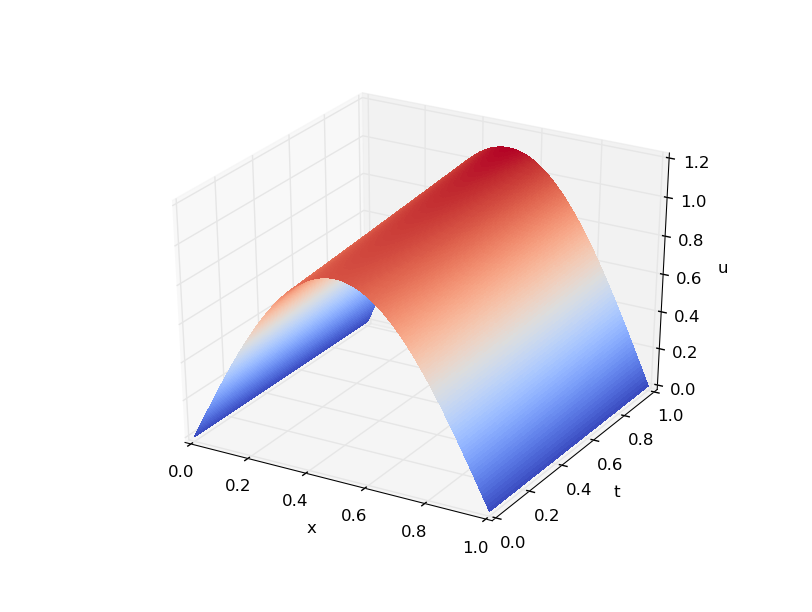
\includegraphics[width=2.4in]{par_ex_pi01}
  \caption{Без управления}
  \label{fig:test1}
\end{minipage}%
\begin{minipage}{.5\textwidth}
  \centering
  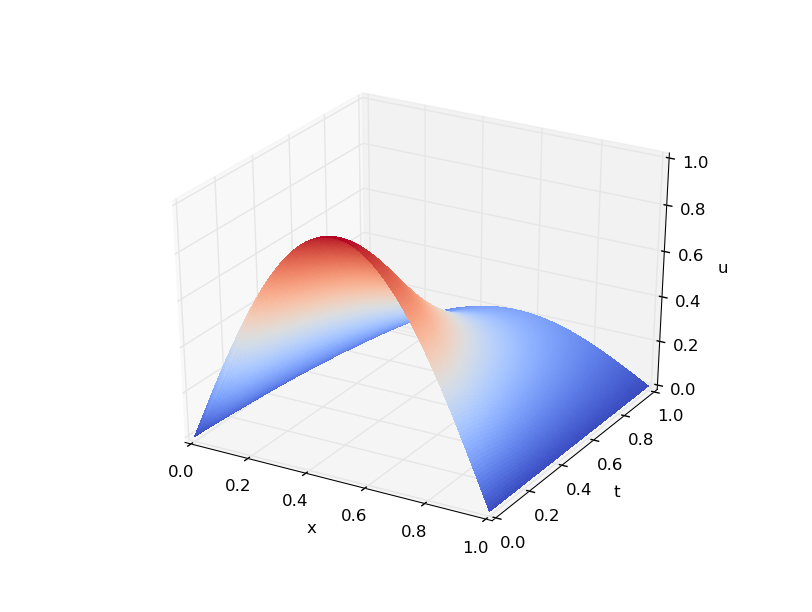
\includegraphics[width=2.4in]{par_re_pi01}
  \caption{$m = 2,\; r = 8$}
  \label{fig:test2}
\end{minipage}
\end{figure}

\end{frame}

\begin{frame}
\frametitle{Пример неустойчивого решения уравнения теплопроводности}

Пусть $u(x, 0) = x(1 - x)$. Фиксируем $\alpha = \pi^2 + 3$, $\omega = (0, 0.4)$.


\begin{figure}[H]
\centering
\begin{minipage}{.5\textwidth}
  \centering
  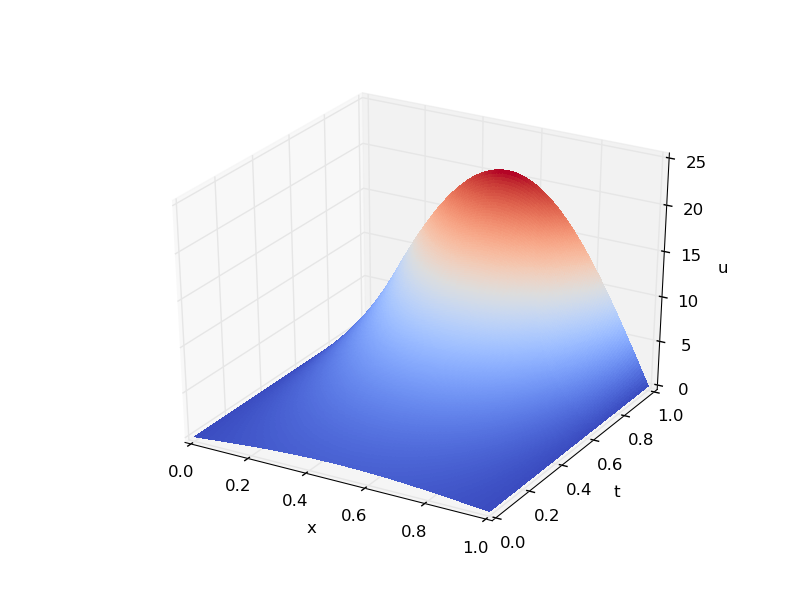
\includegraphics[width=2.4in]{par_ex_pi3}
  \caption{Без управления}
  \label{fig:test1}
\end{minipage}%
\begin{minipage}{.5\textwidth}
  \centering
  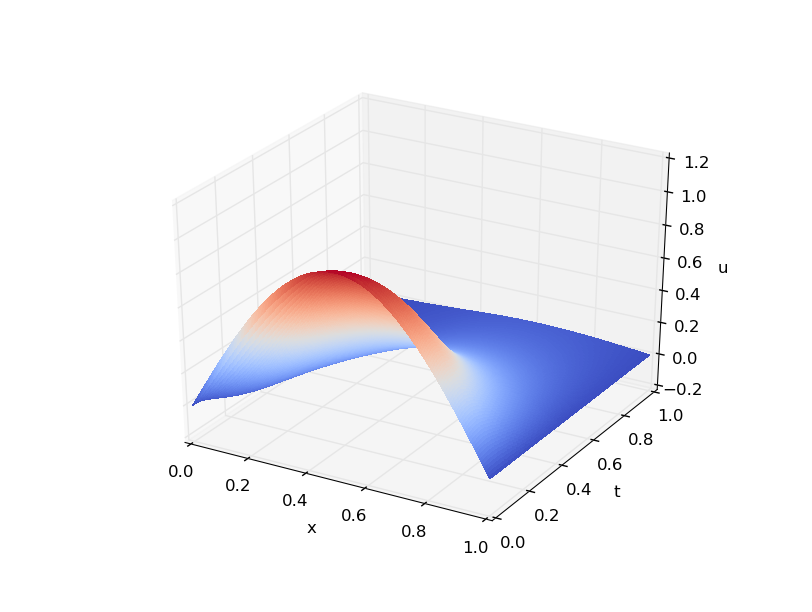
\includegraphics[width=2.4in]{par_re_pi3}
  \caption{$m = 2,\; r = 15$}
  \label{fig:test2}
\end{minipage}
\end{figure}

\end{frame}

\begin{frame}
\frametitle{Стабилизация неустойчивых стационарных решений уравнения Бюргерса}

Рассмотрим вязкое уравнение Бюргерса:
\begin{block}{}

\begin{equation}\label{burger}
    u_t - \nu u_{xx} + u_x u = f + y, \ u|_{\Gamma} = u_b, \quad t > 0.
\end{equation}

\end{block}

Пусть $U$ - стационарное решение \eqref{burger}, то есть

\begin{block}{}
\begin{equation}\label{stationary_sol}
    -\nu U_{xx} + U U_x = f, \ U|_{\Gamma} = u_b,
\end{equation}
\end{block}

Обозначем за $\varphi = u - U$

\end{frame}

\begin{frame}
\frametitle{Стабилизация неустойчивых стационарных решений уравнения Бюргерса}
\textit{Для заданного} $\sigma > 0$ 
\textit{требуется найти оператор управления с обратной связью} 
$y = \Lambda(u - U) : H \to H$ \textit{такой, что} $\mathbf{supp} \ y (\cdot,t) \subset 
\bar{\omega}$ \textit{и}

\begin{block}{}

\begin{gather}\label{fluct}
    \varphi_t - \nu \varphi_{xx} + \varphi U_x + (\varphi + U)\varphi_x =
    \Lambda(\varphi),\\* 
    \varphi|_{\Gamma} = 0, \ t > 0,\\*
    \varphi|_{t = 0} = \varphi_0 = u_0 - U.
\end{gather}
\end{block}
чтобы $\norm{\varphi(t)}_{L^2(\Omega)} \le C e^{-\sigma t}$ при $t \to
+\infty$, если мала норма $\norm{\varphi_0}_{L^2(\Omega)}$

\end{frame}

\begin{frame}
\frametitle{Неустойчивость стационарных решений типа shock-like}

Рассмотрим семейство стационарных решений типа shock-like
\begin{block}{}
\begin{equation}\label{shock_like}
    U(x) = -2\tau\tanh{(\tau(x - \frac{1}{2}))}, \ \text{где } \tau \ge 0.
\end{equation}
\end{block}

\begin{figure}[H]
    \centering
    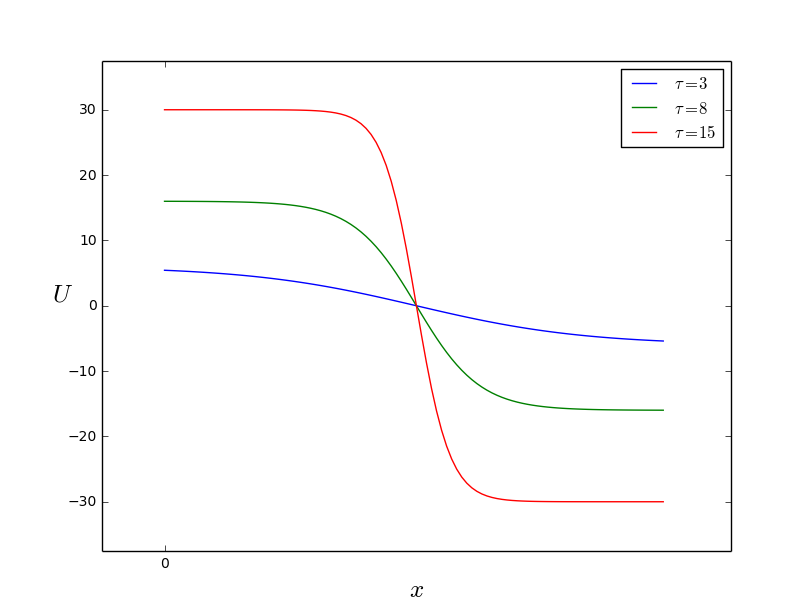
\includegraphics[width=2.5in]{fig1}
    \caption{$U(x)$ при разных $\tau$}
\end{figure}

\end{frame}

\begin{frame}
\frametitle{Неустойчивость стационарных решений типа shock-like}

Для изучения устойчивости системы \eqref{fluct} без стабилизирующего управления, 
мы линеаризуем её

\begin{block}{}
\begin{gather}\label{linearized}
    \theta_t = \theta_{xx} + 2 \tau (\tanh(\tau(x - \frac{1}{2}))\theta)_x, \\*
    \theta(0, t) = \theta(1, t) = 0,
\end{gather}
\end{block}

Избавимся от конвекционого члена используя преобразование 
$\zeta(x, t) = G(x)\theta(x, t)$, где 

\begin{block}{}
\begin{equation}
    G(x) = \frac{\cosh(\tau(x - \frac{1}{2}))}{\cosh(\frac{\tau}{2})}.
\end{equation}
\end{block}

\end{frame}

\begin{frame}
\frametitle{Неустойчивость стационарных решений типа shock-like}

\begin{block}{}
\begin{gather} \label{transf_linear}
    \zeta_t = \zeta_{xx} + \tau^2 \left( \frac{2}{\cosh^2(\tau(x -
    \frac{1}{2}))} - 1 \right) \zeta, \\* 
    \zeta(0) = \zeta(1) = 0.
\end{gather}
\end{block}
Для $\tau = 0$ система нейтрально устойчива. Для $\tau > 0$, коэффициент 
$\mu = \left(\frac{2}{\cosh^2(\tau(x - \frac{1}{2}))} - 1 \right)$  в 
\eqref{transf_linear} является "неустойчивым" в окрестности 
$x = \frac{1}{2}$ (Рис 2.), т.е. положительность этого члена ведет к
неустойчивости системы.

\end{frame}

\begin{frame}
\frametitle{Неустойчивость стационарных решений типа shock-like}

\begin{figure}[H]
    \centering
    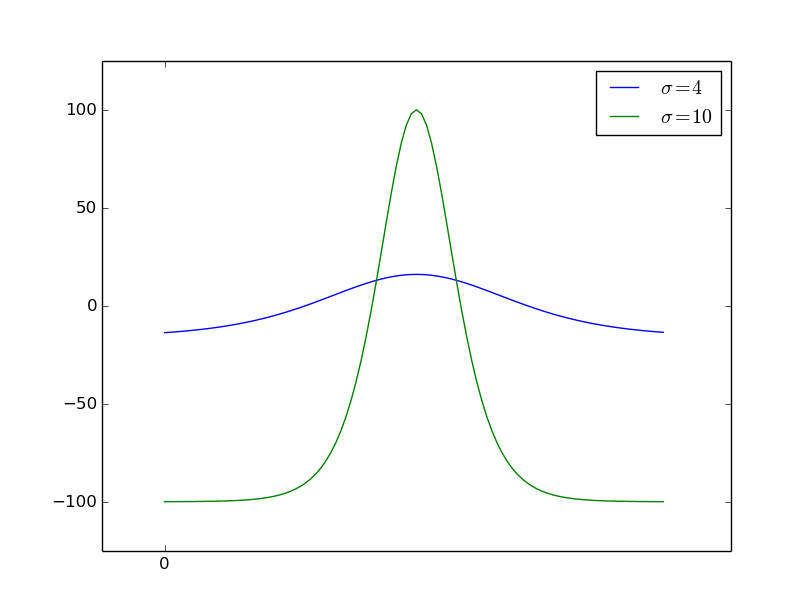
\includegraphics[width=3.5in]{fig2}
    \caption{График $\mu$ в \eqref{transf_linear}}
\end{figure}

\end{frame}

\begin{frame}
\frametitle{Примеры неустойчивых стационарных решений}

Начальное условие $\theta_0(x) = \frac{\sin(\pi x)}{G(x)}$, параметр $\tau$ 
возмем равный 15. На рис. 7 показано неустойчивое поведение системы
\eqref{fluct}

\begin{figure}[H]
    \centering
    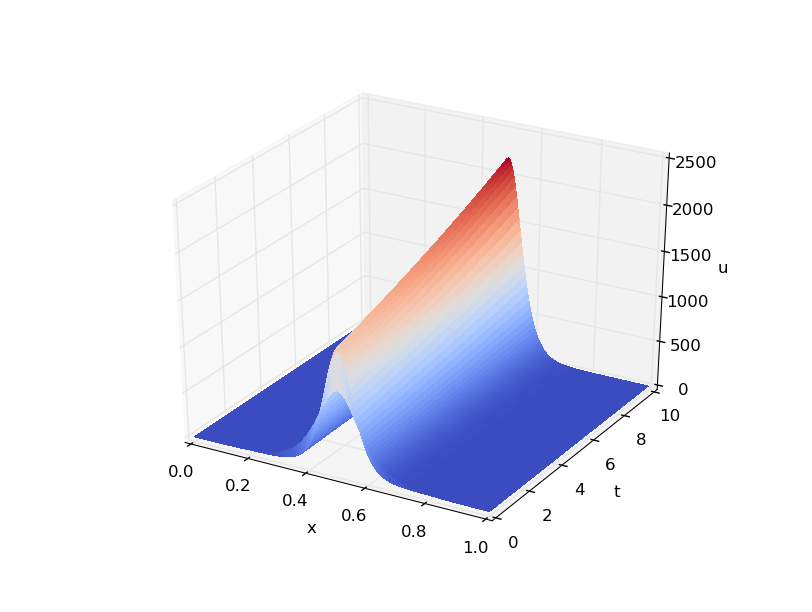
\includegraphics[width=3in]{ex_s15}
    \caption{}
\end{figure}

\end{frame}

\begin{frame}
\frametitle{Примеры неустойчивых стационарных решений}

Начальное условия $\theta_0(x) = \frac{x^2}{G(x)}$. Параметр $\tau = 15$.
Поведение решения представлено на рис.8.

\begin{figure}[H]
    \centering
    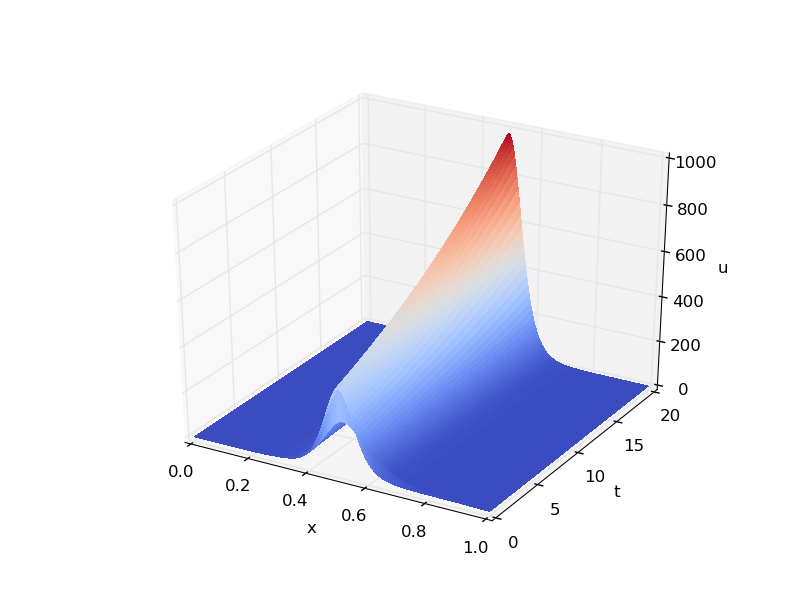
\includegraphics[width=3in]{ex_x2_s15}
    \caption{}
\end{figure}

\end{frame}

\begin{frame}
\frametitle{Конструкция управления}

Оператор стабилизирующего управления имеет следующую структуру

\begin{block}{}
\begin{equation}
    \Lambda(\varphi) = -r \chi_{\omega}h(\mu)P\varphi.
\end{equation}
\end{block}

Здесь $\mu = \norm{P_m\varphi} - 2 \norm{Q_m\varphi}$

\begin{block}{}
\begin{gather*}
    \begin{matrix}
        h(\mu) & =
        & \left\{
        \begin{matrix}
            0, & \mu < 0, \\
            1, & \mu > 0, \\
            [0, 1], & \mu = 0
        \end{matrix} \right.
    \end{matrix} \quad
    \begin{matrix}
        \chi_{\omega}(x) & =
        & \left\{
        \begin{matrix}
            0, & \mbox{если } x \notin \omega, \\
            1, & \mbox{иначе. }
        \end{matrix} \right.
    \end{matrix}
\end{gather*}
\end{block}
$r > 0$, $\chi_{\omega}$ - характеристическая функция области $\omega$,
$h(\mu)$ - многозначная функция Хевисайда\\

\end{frame}

\begin{frame}
\frametitle{Конечномерная стабилизация}

\begin{block}{}
\begin{equation}\label{final}
    \norm{u(t) - U}^2 \le C e^{-\sigma t}, \ t > 0
\end{equation}
\end{block}

Достаточноые условия на параметры задачи, гарантирующие выполнение \eqref{final}
имеют вид:

\begin{block}{}
\begin{gather*}
    10C_1 \lambda_{m + 1}^{-1} < \nu, \ C_1 = \sigma + \frac{1}{2}
    \norm{U_x}_{L^{\infty}(\Omega)} \\*
    r\gamma \ge C_2, \ C2 = (2 + \gamma)\sigma - \frac{9C_0^2}{4\nu}(1 + \gamma)
\end{gather*}
\end{block}

\end{frame}

\begin{frame}
\frametitle{Примеры численного моделирования стабилизации}

Пусть $\theta_0 = \frac{sin(\pi x)}{G(x)}$ - начальное условие, $\tau = 15$
- параметр семейства shock-like

\begin{figure}[H]
  \centering
  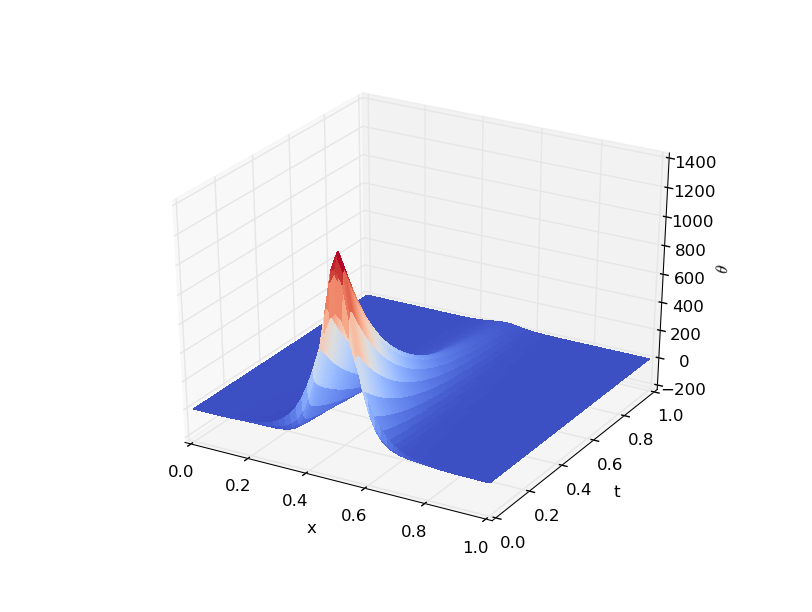
\includegraphics[width=3in]{re_s15}
  \caption{Управление с $\omega = (0, 0.4), \; m = 4, \; r = 30$}
  \label{fig:test2}
\end{figure}

\end{frame}

\begin{frame}
\frametitle{Примеры численного моделирования стабилизации}

Начальное условие $\theta_0(x) = \frac{x^2}{G(x)}$, $\tau = 15$.

\begin{figure}[H]
 \centering
  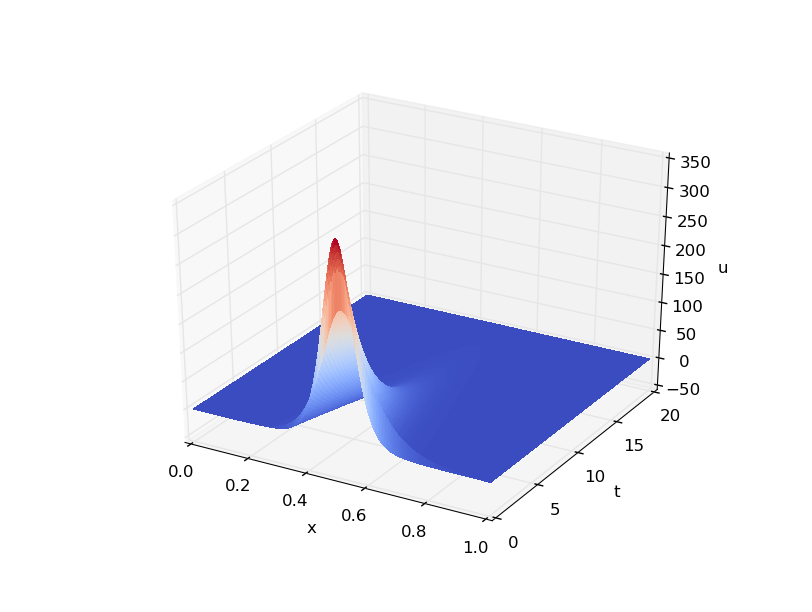
\includegraphics[width=3.0in]{re_x2_s15}
  \caption{$\omega = (0, 0.4), \; r = 30, \; m = 3$}
  \label{fig:test2}
\end{figure}

\end{frame}


\begin{frame}
\frametitle{Заключение}

В представленной ВКР предложен простой метод стабилизации неустойчивых
стационарных решений параболических уравнений. Особенность предложенного
алгоритма заключается в локальности носителя управления и конечномерности образа
оператора управления. В работе разработан алгоритм реаллизации стабилизирующего
управления для линейного уравнения теплопроводности и нелинейного уравнения
Бюргерса, в том числе написание программы для решения разностных схем и
реализация метода Филона для интегралов от быстро осциллирующих функций.
Приведены численные примеры неустойчивых стационарных решений параболических
уравнений, и "применение" предложенного метода стабилизации.

\end{frame}

\begin{frame}
	\begin{center}
	\Huge Спасибо за внимание
	\end{center}
\end{frame}

\end{document}
